\documentclass[12pt]{beamer}

\usepackage[size = a0, orientation = portrait, scale = 1.5]{beamerposter}

\usefonttheme{serif}

\usepackage[english]{babel}
\usepackage[utf8x]{inputenc}
\usepackage[T1]{fontenc}
\usepackage{lmodern}
\usepackage{indentfirst}
\usepackage{ragged2e}
\usepackage[]{natbib} 
\usepackage{graphicx}
\usepackage{animate}
\usepackage{color}
\usepackage{colortbl}

% For 'InkScape' integration
\usepackage{import}
\usepackage{xifthen}
\usepackage{pdfpages}
\usepackage{transparent}

\setbeamertemplate{navigation symbols}{}
\setbeamertemplate{caption}[numbered]

\definecolor{title-bg}{RGB}{240, 240, 240}
\definecolor{title-fg}{RGB}{128, 113, 93}
\definecolor{my-red}{RGB}{254, 132, 135}
\definecolor{my-blue}{RGB}{59, 180, 252}
\definecolor{my-green}{RGB}{125, 221, 149}
\definecolor{titles}{RGB}{0, 166, 160}
\setbeamercolor{block title}{fg = title-fg, bg = title-bg}
\setbeamercolor{header-color}{fg = title-fg, bg = title-bg}

\setbeamertemplate{headline}{%
\begin{beamercolorbox}[wd=1.00\textwidth]{header-color}
	\begin{columns}[T]
		\begin{column}{0.235\textwidth}
			
\includegraphics[width=1.15\linewidth]{Images/KAUST_logo}
		\end{column}
		\begin{column}{0.765\textwidth}
			\vspace{32pt}
			\begin{beamercolorbox}[wd=1.00\textwidth]{header-color}	
			{\Large Modeling Infectious Disease Dynamics: Integrating Contact Tracing-based Stochastic Compartment and Spatio-temporal Risk Models \par} \vspace{12pt}
			
			{\normalsize
				André Victor Ribeiro Amaral${\phantom{|}}^{1, \star}$, 
				Mateen Mahmood${\phantom{|}}^{1}$,
				Jorge Mateu${\phantom{|}}^{2}$, and 
				Paula Moraga${\phantom{|}}^{1}$
			}	\vspace{16pt}
		
			{\footnotesize
			${}^{1}\hspace{8pt}$Computer, Electrical and Mathematical Sciences and Engineering Division, King Abdullah University of Science and Technology (KAUST). Kingdom of Saudi Arabia. \\ \vspace{3pt}
			${}^{2}\hspace{8pt}$Department of Mathematics, Universitat Jaume I. Spain. \\ \vspace{10pt}
			${}^{\star}$ E-mail: \texttt{andre.ribeiroamaral@kaust.edu.sa}
			}
		
		
			\end{beamercolorbox}
			\vspace{24pt}
		\end{column}
	\end{columns}
\end{beamercolorbox}
}
\setbeamertemplate{footline}{}

\begin{document}
	\begin{frame}[t]
		\begin{columns}[t]
			%======================================== FIRST COLUMN ========================================
			\begin{column}{0.30\textwidth} \justifying % FIRST COLUMN
				\begin{block}{\Large 1. Introduction} \justifying \vspace{12pt}
					
					Major infectious diseases such as COVID-19 have a significant impact on population lives and put enormous pressure on healthcare systems globally. Strong interventions imposed to prevent these diseases from spreading may also impact society---making crucial the prioritization \hspace{-3pt}of \hspace{-3pt}risky\hspace{-2pt} areas\hspace{-2pt} when\hspace{-2pt} applying \hspace{-3pt}these \hspace{-2pt}protocols.\vspace{12pt}
					
					In this work, we propose a new spatial-stochastic model that allows us to characterize the temporally varying spatial risk better than existing methods. This is achieved by taking advantage of (the recently available) \textit{Contact-tracing data}, i.e., data collected from the process of identifying individuals' previous infected contacts aiming to test, isolate and trace them.\vspace{12pt}
					
					\begin{figure}[!ht]
						\centering
						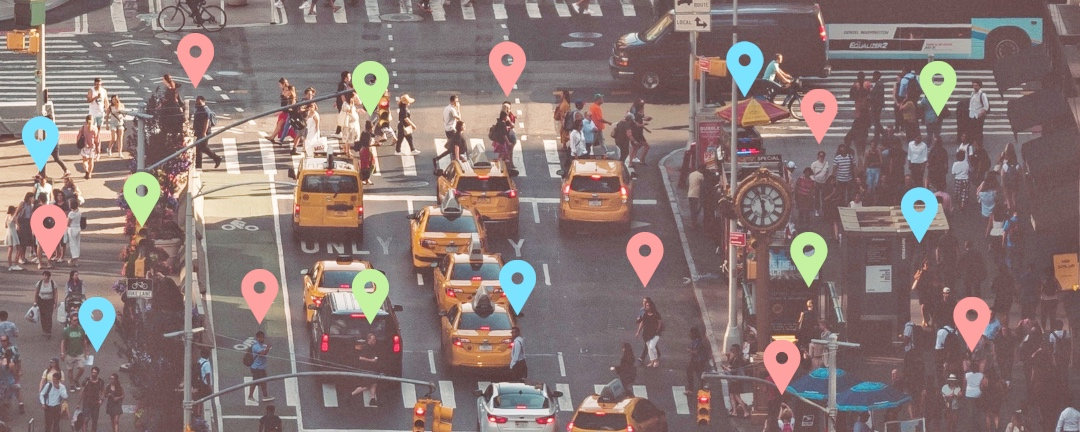
\includegraphics[width = 1\textwidth]{Images/SIR_image}
						\caption{\justifying Illustration of Contact-Tracing data with labeled\hspace{-1pt} \textcolor{my-blue}{\textbf{Susceptible}}, \textcolor{my-red}{\textbf{Infected}}, and \textcolor{my-green}{\textbf{Recovered}} people.}
						\label{fig:SIR-illustration}
					\end{figure}
				
				\end{block} 
			
			\begin{block}{\Large 2. Methodology}\justifying \vspace{12pt}
				
				
			{\large \textcolor{title-fg}{Base-SIR modeling}} \vspace{12pt}
			
			In this base-SIR model \cite{hernandez2020evaluating}, assuming a closed environment, there are five different compartments where an individual can be during an epidemic, which represent the states of Susceptible (S), Infected (I), Recovered (R), Quarantine Susceptible ($\text{Q}_\text{S}$), and Quarantine Infected ($\text{Q}_\text{I}$). Also, an individual can be transferred from one compartment to another in seven different ways, namely: $\text{S}\rightarrow\text{I}$, $\text{S}\rightarrow\text{Q}_{\text{S}}$, $\text{S}\rightarrow\text{Q}_{\text{I}}$, $\text{I}\rightarrow\text{Q}_{\text{I}}$, $\text{Q}_{\text{S}}\rightarrow\text{S}$, $\text{I}\rightarrow\text{R}$, and $\text{Q}_{\text{I}}\rightarrow\text{R}$ (Figure \ref{fig:base-SIR}). \vspace{18pt}
			
			\begin{figure}[!ht]
				\centering
				\def\svgwidth{\columnwidth}\import{./Images/inkscape}{blocks.pdf_tex}
				\caption{\justifying All 5 compartments and the 7 possible transfers.}
				\label{fig:base-SIR}
			\end{figure}
		
			The epidemic dynamic is control by parameters from Table \ref{table:parameters-SIR}.
			
			\begin{table}[!ht]
				\centering
				\caption{\justifying Description of compartment model parameters.}\vspace{-24pt}
				\resizebox{\textwidth}{!}{%
					\begin{tabular}{c|l}
						Parameter & \multicolumn{1}{c}{Description} \\ \hline
						$\kappa$ & Average degree (daily contacts per individual) \\ 
						$\mathcal{K}_i$& Contacts of individual $i$ with infected individuals \\
						$\mathcal{R}_0$&  Basic reproductive ratio \\
						$\delta$ & Rate of detection \\
						$\gamma$ & Recovery rate \\
						$b$ & Probability of transmission of infection\\
						$\tau_Q$& Time in quarantine  \\
						$\mathcal{C}_i(\triangle)$ & Backward contact tracing of individual $i$ with detected infected individuals 
					\end{tabular}%
				}
				\label{table:parameters-SIR}
			\end{table}

			Extending the base-SIR model, we can  incorporate the idea of \textit{temporally varying spatial risk} \cite{mahmood2021contextual}. This approach consists in computing a \textit{risk value} for each piece of the total considered area, which will play an important role in how some model parameters are updated in each round of this iterative process. 
			
			\end{block}
				
			\end{column}
		
			%======================================== SECOND COLUMN ========================================
			\begin{column}{0.30\textwidth} \justifying % SECOND COLUMN
				
			{\large \textcolor{title-fg}{New spatio-temporal-SIR modeling}} \vspace{12pt}
			
			Here, we propose a new stochastic-spatial model to better characterize the spatial risk. \vspace{12pt}
			
			For each cell of the studied region, the Relative Risk (RR) will be used to update a quantity that tracks the contacts among individuals in such a way that it will flag if two pedestrians have interacted within that particular cell, and later, it will be used to update the rate equations---used to model the pedestrians' transfers among compartments (Figure \ref{fig:rr-modeling}).\vspace{12pt}
			
			\begin{figure}[!ht]
				\centering
				\def\svgwidth{\columnwidth}\import{./Images/inkscape}{diagram2.pdf_tex}
				\caption{\justifying Relative Risk model from Contact-tracing data.}
				\label{fig:rr-modeling}
			\end{figure}
			
			Formally, for $Y_j$ representing the number of contacts between one infected and one susceptible person in a cell $j$, we set 
			\begin{align*}\label{eq:model-RR}
				Y_j \sim \text{Poisson}(E_j\cdot\theta_j), \text{~for all~} j
			\end{align*}
			where $\log(\theta_j) = \beta_0 + \beta_1 \cdot x_{1j} + u_j$, such that $x_{1j}$ represents the number of buildings (or another factor affecting risk) in $j$, and $u_j \overset{\text{i.i.d.}}{\sim} \text{Normal}(0, \sigma^2_{u})$ \cite{moraga2019geospatial}. Also, for $c^{is}_{j}$ corresponding to the number of contacts between an infected person and a susceptible one, $c^{ii}_{j}$ to the number of contacts between two infected people, and $c^{ss}_{j}$ to the number of contacts between two susceptible people, 	$E_j = (\texttt{pop}_j \cdot \theta_{\text{all}})$, such that $\texttt{pop}_j = (c^{is}_{j} + c^{ii}_{j} + c^{ss}_{j})$, and 
			\begin{align*} % Reference: https://tex.stackexchange.com/questions/252354/sum-symbol-in-tikzposter-too-small
				\theta_{\text{all}} = \frac{\displaystyle\raisebox{-18pt}{\scalebox{3.2}{\ensuremath{\sum}}}_{\text{all} j}Y_j}{\displaystyle\raisebox{-18pt}{\scalebox{3.2}{\ensuremath{\sum}}}_{\text{all} j}\texttt{pop}_j}.
			\end{align*}
			Finally, as we may not observe contacts in many different cells, there is no reason to believe that these regions are more or less risky than the overall considered area. Therefore, if $\texttt{pop}_j = 0$ for some $j$, we set $\text{RR}_j$ to 1.\vspace{12pt}
		
			\begin{block}{\Large 3. Simulation}\justifying \vspace{12pt}
				
				{\large \textcolor{title-fg}{Mobility data simulation}} \vspace{12pt}
				
				Using the \texttt{Simulation of Urban Mobility} (SUMO) software \citep{SUMO2018}, we simulated  the movement of 1,000 pedestrians across the city of Valencia, Spain, for 150 days.\vspace{12pt}
				
				\begin{figure}[!ht]
					\centering
					
					\vspace{-18pt}
					
					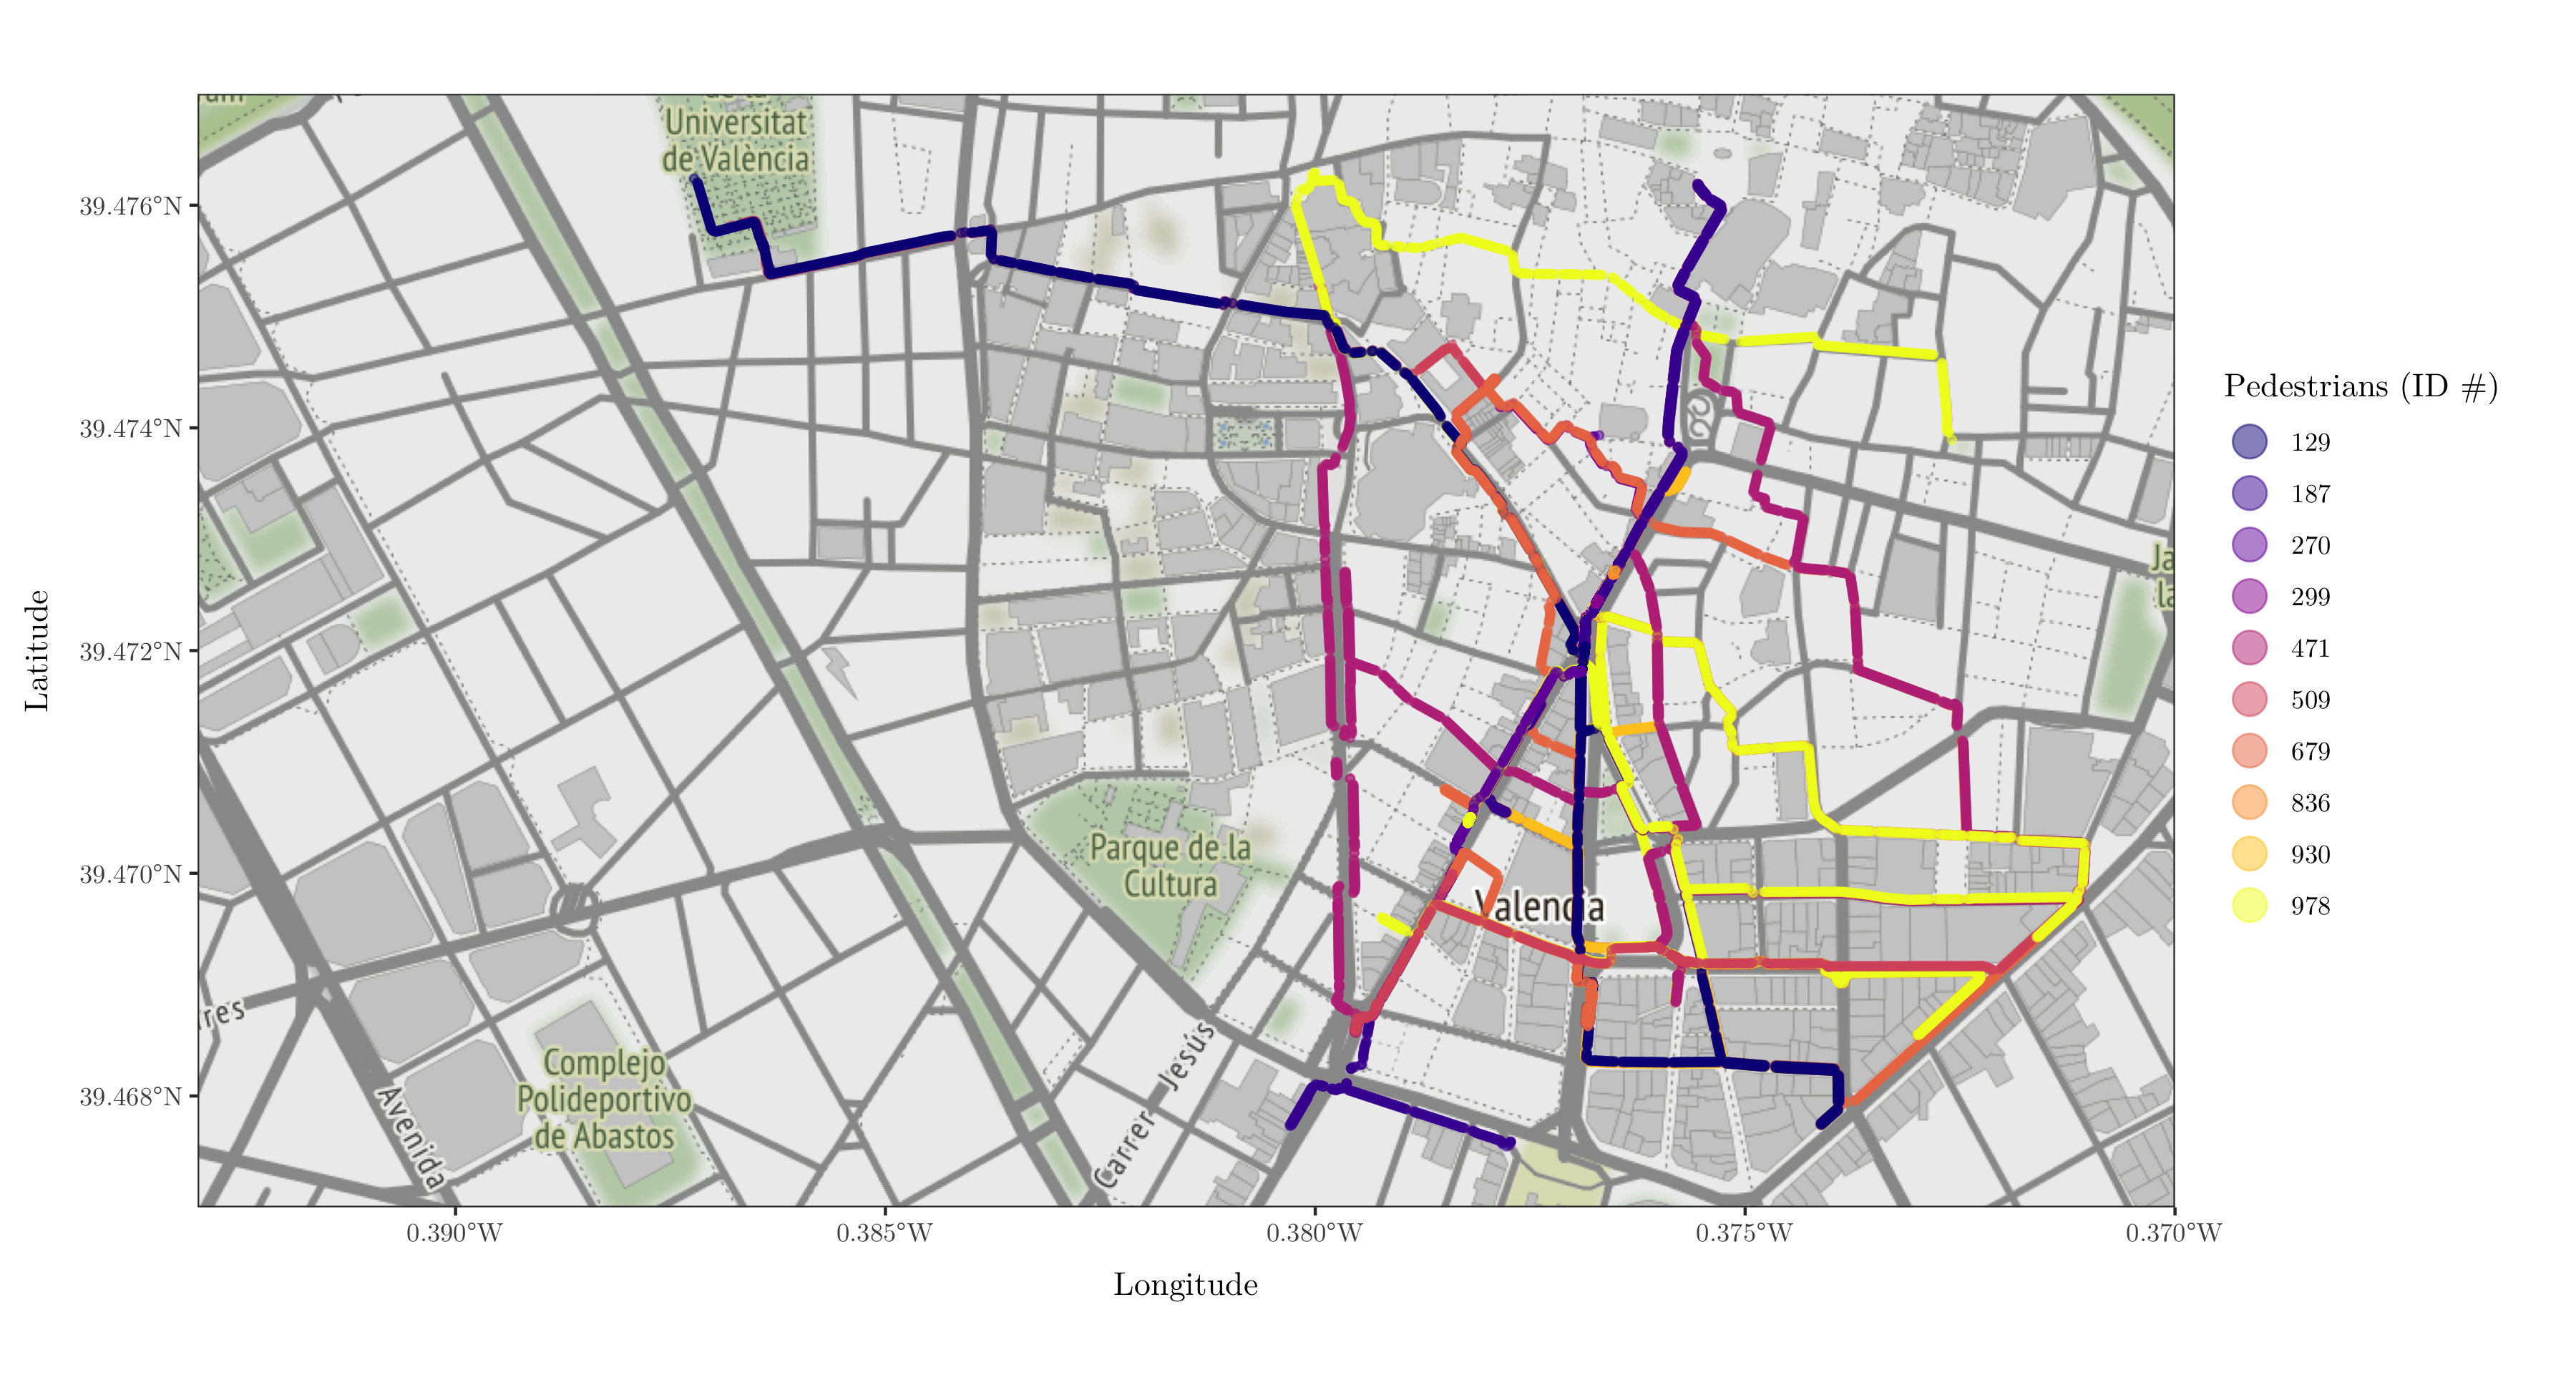
\includegraphics[width = 1\textwidth]{Images/pedestrians}
					
					\vspace{-24pt}
					
					\caption{\justifying SUMO Simulated trajectory for 10 randomly selected pedestrians in the ``day 1'' in Valencia. ``\texttt{ID \#}'' refers to the pedestrian code number in the data set.}
					\label{fig:pedestrians}
				\end{figure}\vspace{-3pt}
				
				
				The region from Figure \ref{fig:pedestrians} was divided into 230 cells and, aiming at increasing the number of contacts, 23 cells (same cells with high building density) were set as \textit{high priority} (Figure \ref{fig:buildings-contacts}).\vspace{12pt}

			\end{block}
			
			
			\end{column}
		
			%======================================== THIRD COLUMN ========================================
			\begin{column}{0.30\textwidth} \justifying % THIRD COLUMN
				
				\vspace{-10pt}
				\begin{figure}[!ht]
					\centering
					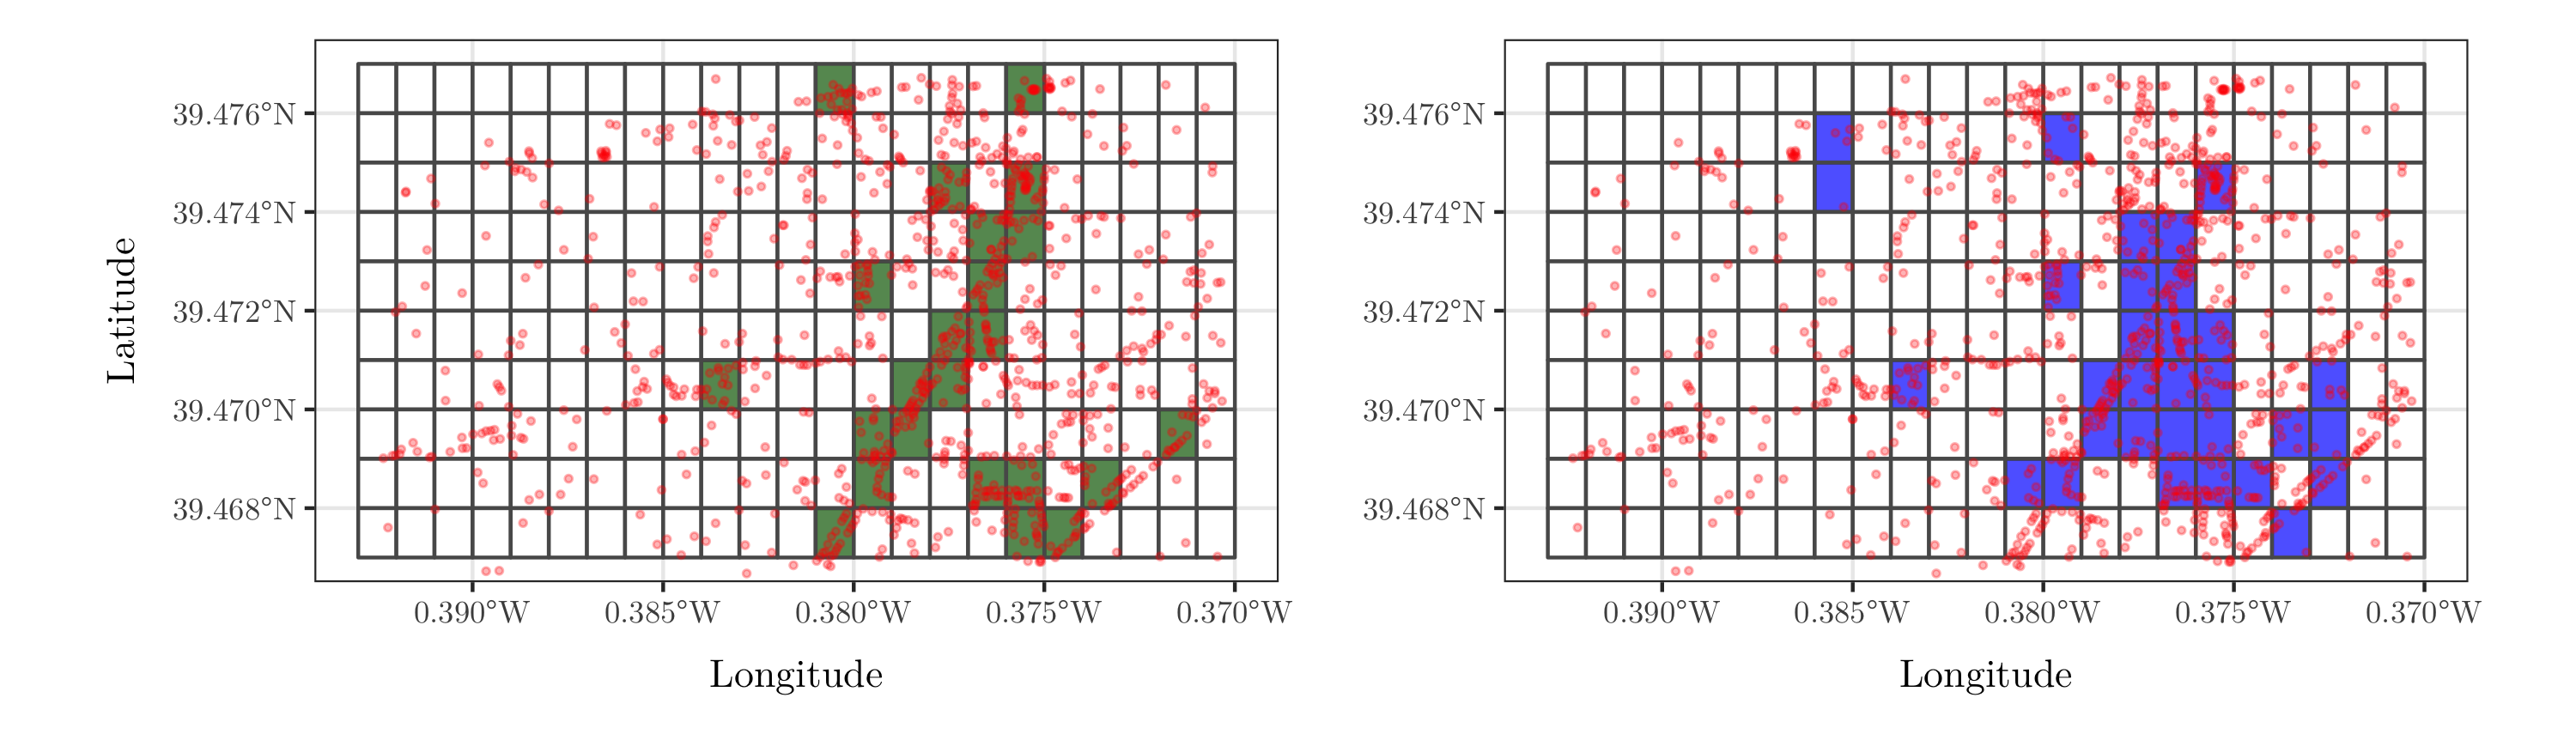
\includegraphics[width = 1\textwidth]{Images/buildings-contacts}
					\caption{\justifying 23 selected cells (left), and cells where at least one contact occurred (right). Red dots are the buildings.}
					\label{fig:buildings-contacts}
				\end{figure}\vspace{-6pt}
				
				For the same simulated data set, we fit and compare the results obtained with the base-SIR and the new spatio-temporal-SIR models.\vspace{18pt}
			
				{\large \textcolor{title-fg}{Base-SIR fitted model}} \vspace{12pt}
				
				For a set of initial values \cite{hernandez2020evaluating}, Figure \ref{fig:fitted-base} shows the simulated process for the base-SIR model.
				
				\begin{figure}[!ht]
					\centering
					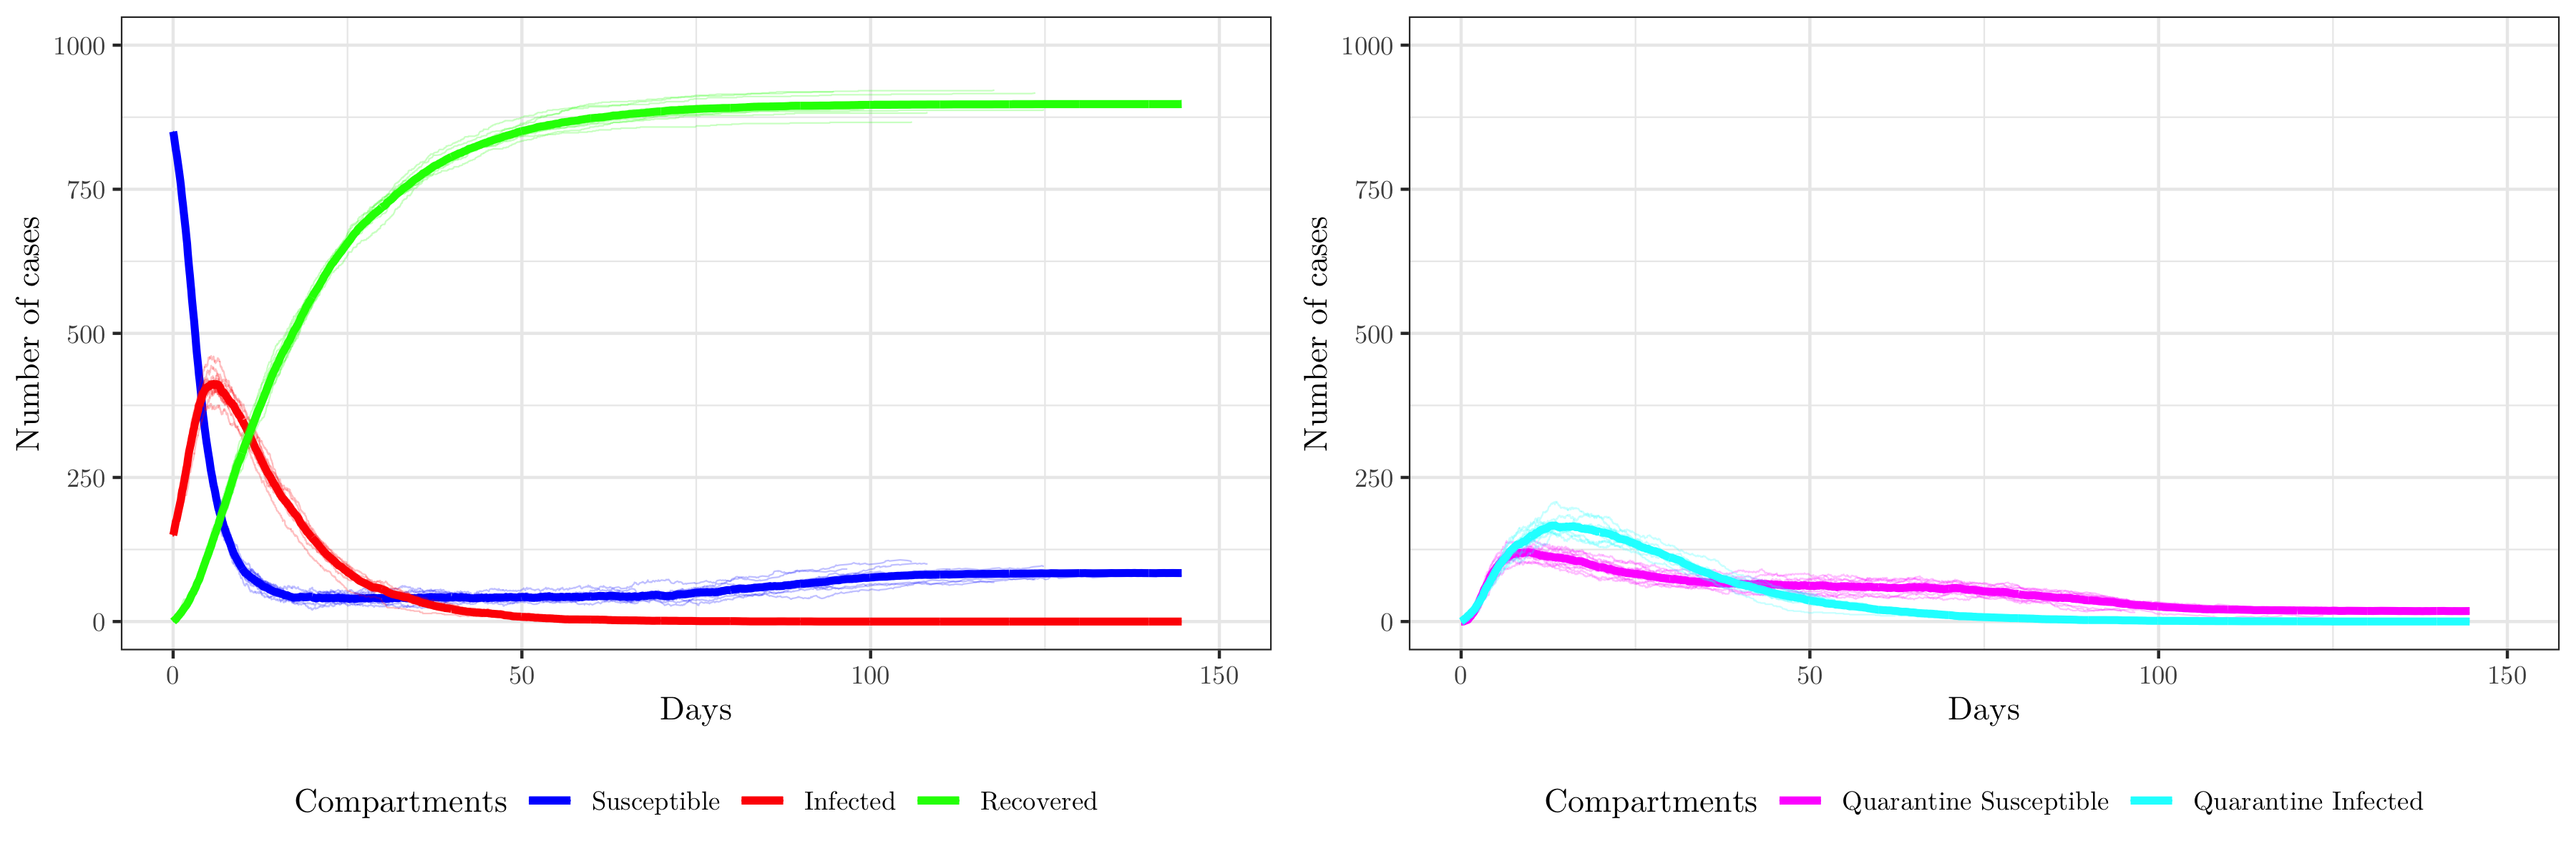
\includegraphics[width = 1\textwidth]{Images/fitted-base}
					\caption{\justifying Simulated number of individuals using the \textbf{base-SIR model}. Light lines represent 10 realizations of the epidemic, and the bold lines their mean.}
					\label{fig:fitted-base}
				\end{figure}\vspace{-6pt}
				
				{\large \textcolor{title-fg}{New spatio-temporal-SIR fitted model}} \vspace{12pt}
				
				Before simulating the pandemic, first, we have to estimate $\text{RR}_j$, for all $j$ and all time-windows.
				
				\begin{figure}[!ht]
					\centering
					%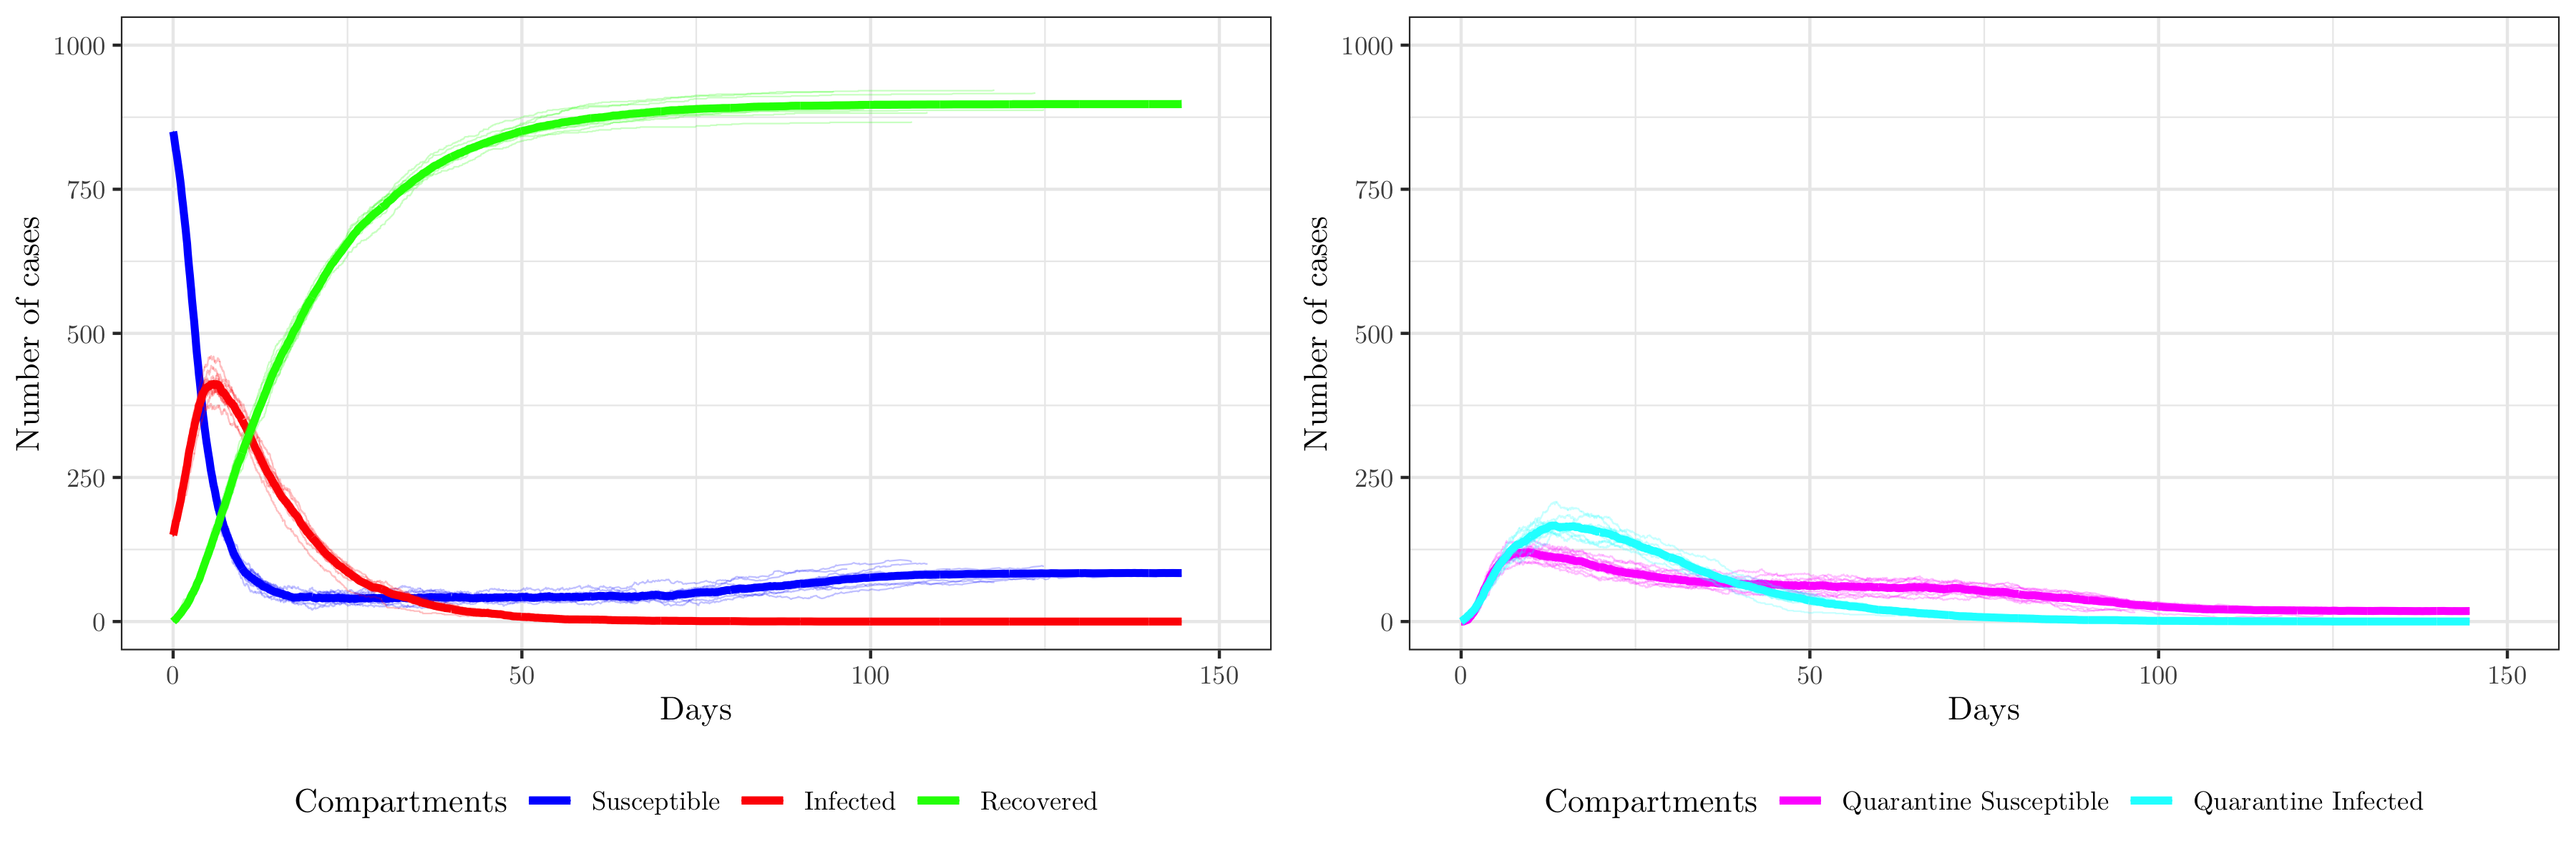
\includegraphics[width = 1\textwidth]{Images/fitted-base}
					\animategraphics[loop, controls = {play, stop}, width=0.80\linewidth, buttonsize = 20pt]{4}{Images/Animation/window}{1}{4} % UPDATE IT FOR THE PRESENTATION
					\vspace{6pt}
					\caption{\justifying Animation for the estimated Relative Risks for all 230 cells in the second window of days 1, 2, 3, and 4.}
					\label{fig:estimated-rr}
				\end{figure}\vspace{-12pt}
			
				Then, for the same set of initial values as before, we can fit the new spatio-temporal-SIR model.
				
				\begin{figure}[!ht]
					\centering
					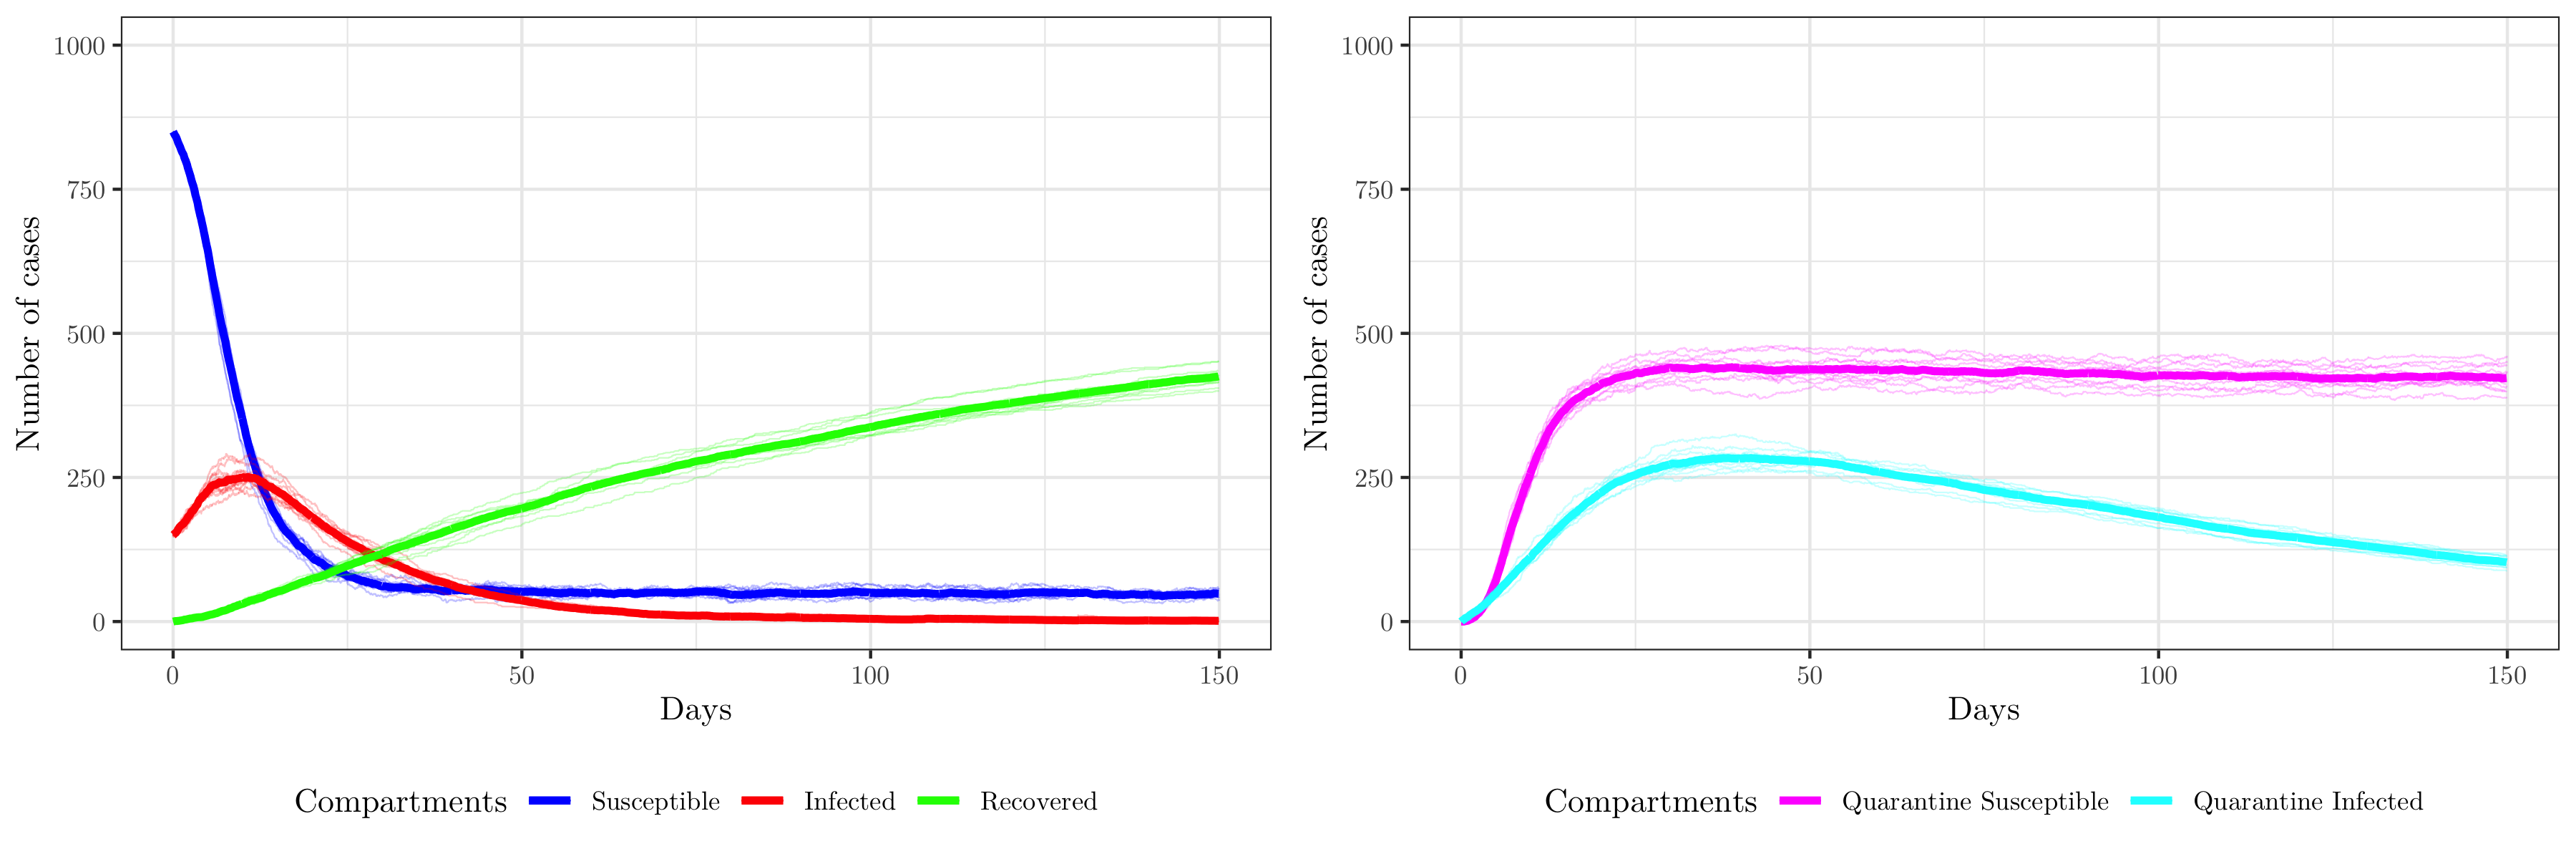
\includegraphics[width = 1\textwidth]{Images/fitted-temporal}
					\caption{\justifying Simulated number of individuals using the \textbf{spatio-temporal-SIR model}. Light lines represent 10 realizations of the epidemic, and bold lines their mean.}
					\label{fig:fitted-temporal}
				\end{figure}\vspace{-6pt}
			
			With our new model,  since riskier areas affect more the disease transmission, people who visited these places were quarantined and the peak of the epidemic was reduced.\vspace{12pt}
			
			\begin{block}{\Large 4. Conclusion}\justifying \vspace{12pt}
				
				The integration of stochastic compartment and spatial risk models helps us to better understand the epidemic dynamics. Also, this approach helps policymakers to develop strategies that may prevent individuals from visiting riskier areas and contributing to disease spread.\vspace{12pt} 
				
			    This work provides a framework that allows us to make the best use of real-time data to combat infectious diseases and promote sustainability.\vspace{12pt} 
				
				%Keeping track of individuals' movements  may help decision-makers understanding the population contact patterns and, based on this acquired knowledge, propose policies that may prevent individuals from visiting riskier areas and contributing to the disease spreading. \vspace{12pt} 
				
				%And the obtained results showed that introducing a Relative Risk model into our framework might\hspace{-2pt} contribute\hspace{-2pt} to\hspace{-2pt} the\hspace{-2pt} epidemic\hspace{-2pt} peak\hspace{-2pt} reduction.\vspace{12pt} 
			\end{block}
		
		\begin{block}{References}\justifying \vspace{12pt}\tiny

				\bibliographystyle{plain}
				\bibliography{References/References}
		\end{block}	
				
			\end{column}
		\end{columns}
	\end{frame}

%
%
%	\begin{frame}[t]
%	\begin{columns}[t]
%		%======================================== FIRST COLUMN ========================================
%		\begin{column}{0.30\textwidth} \justifying % FIRST COLUMN
%			
%				\begin{block}{\Large 4. Conclusion}\justifying \vspace{12pt}
%				Keeping track of individuals' movements  may help decision-makers understanding the population contact patterns and, based on this acquired knowledge, propose policies that may prevent individuals from visiting riskier areas and contributing to the disease spreading. \vspace{12pt} 
%				
%				Also, the obtained results show that the introduction of the estimated Relative Risk values into the model may contribute to the reduction of the epidemic peak. \vspace{12pt} 
%			\end{block}
%			
%			\begin{block}{\Large References}\justifying \vspace{12pt} \scriptsize
%				\bibliographystyle{plain}
%				\bibliography{References/References}
%			\end{block}	
%				
%				
%
%
%
%
%
%{\normalsize \textcolor{title-fg}{~~Simulation of pedestrian mobility}} \vspace{12pt}
%
%Due to the difficulty in obtaining real-world mobility data, we opted for simulating pedestrians' movement across a selected region. This simulation process is performed using the software named  \texttt{Simulation of Urban Mobility} (SUMO) \citep{SUMO2018}. For a given region (city of Valencia, in Spain), we are able to generate map-matched trajectory data for people walking on streets during a specific time-window. \vspace{12pt}
%
%				
%		\end{column}
%		
%		%======================================== SECOND COLUMN ========================================
%		\begin{column}{0.30\textwidth} \justifying % SECOND COLUMN
%
%		\end{column}
%		
%		%======================================== THIRD COLUMN ========================================
%		\begin{column}{0.30\textwidth} \justifying % THIRD COLUMN
%
%		\end{column}
%	\end{columns}
%\end{frame}
%
%
\end{document}